\chapter{Domain Driven Design}
\section{Ubiquitous Language}
In \ref{table} wird die Ubiquitous Language der Domäne analysiert.
\begin{table}[]
    \begin{tabular}{|l|l|}
    \hline
    \textbf{Wort} & \textbf{Bedeutung} \\ \hline
    User & Ein User stellt eine Person dar, die ihre Konten verwalten möchte \\ \hline
    Konto & Ein Konto stellt eine Einheit dar, auf der Geld gespeichert wird \\ \hline
    Transaktion & \begin{tabular}[c]{@{}l@{}}Eine Transaktion ist ein Auftrag, der von einem Konto ausgeht \\ oder dieses betrifft. \\ Dies stellt beispielsweise eine Überweisung dar\end{tabular} \\ \hline
    Bank & \begin{tabular}[c]{@{}l@{}}Eine Bank ist ein Institu, das Konten von Personen hält und für diese \\ Personen Transaktionen ausführt\end{tabular} \\ \hline
    Anmelden / Login & Ein bereits registrierter User meldet sich an einem System an \\ \hline
    Registrieren & Eine Person erstellt sich einen User in einem System \\ \hline
    Adresse & \begin{tabular}[c]{@{}l@{}}Durch eine Adresse kann eindeutig identifiziert werden, \\ wo sich in dieser Domäne eine Bank befindet oder ein User lebt\end{tabular} \\ \hline
    Kontostand ändern & \begin{tabular}[c]{@{}l@{}}Das Geld, das auf einem Konto gespeichert ist, \\ wird entweder erhöht oder verringert\end{tabular} \\ \hline
    überweisen & \begin{tabular}[c]{@{}l@{}}Beim Überweisen wird eine transaktion erstellt, \\ die Geld von einem Konto auf ein anderes\\ überträgt\end{tabular} \\ \hline
    \end{tabular}
    \label{table}
\end{table}
\section{Analyse und Begründung der verwendeten muster des DDD}
\subsection{Value Objects (VO)}
Value Objects oder auch Wertobjekte sind Objekte, die unveränderbar sind. Diese werden einmal erstellt und sind daraufhin nichtmehr änderbar, da sie spezielle Werte repräsentieren. Sie besitzen keine Methoden, da sie nur auf ihre Werte reduziert werden.
Soll der Wert eines Value Objects doch geändert werden, müssen diese neu erstellt werden. In diesem Programmentwurf wurden Value Objects zum einen für die Adresse einer Bank erstellt und zum anderen für die Informationen einer Transaktion. 
Die Adresse ist ein gutes Beispiel für ein Value Object, da sich die Adresse einer Bank später normalerweise nicht ändert, außer die komplette Bank zieht in ein anderes Gebäude um. Dies geschieht jedoch nicht so häufig, dass die 
Adresse änderbar sein muss. Auch die Informationen einer Transaktion sollten unveränderbar sein, damit immer nachvollzogen werden kann, welcher Betrag von welchem Konto auf welches Konto überwiesen wurde. 
\newline In \ref{valueObject} wird ein Ausschnitt aus dem Adressen Value Object gezeigt:
\begin{figure}[htbp]
    \centering
    \fbox{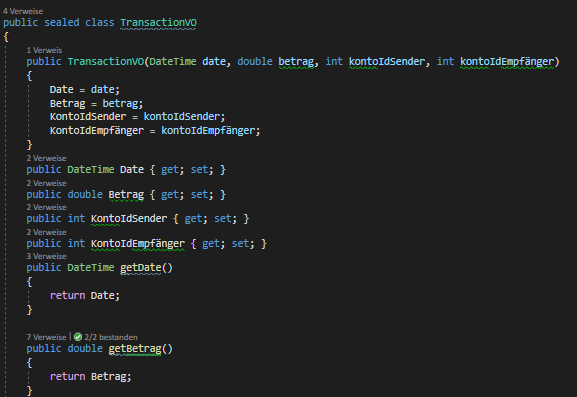
\includegraphics[width=10cm]{voAusschnitt.png}}
    \caption{\label{valueObject} AdressVO}
\end{figure}
\subsection{Entities}
Entities unterscheiden sich in den folgenden 3 Punkten von Value Objects:
\begin{itemize}
    \item Entities haben eine eindeutige Id
    \item Wenn Entities unterschiedliche Ids haben unterscheiden sie sich voneinander
    \item Eine Entity hat einen Lebenszyklus und verändert sich während diesem Zyklus häufiger
\end{itemize}
Es wurden in diesem Projekt folgende Entitäten angelegt:
\begin{itemize}
    \item User
    \item Konten
    \item Banken
\end{itemize}
Diese sind eindeutige Objekte die unterschieden werden müssen. Sie können sich von Zeit zu Zeit verändern. Vorallem Konten verändern sich häufig, da immer wieder Geld auf ein Konto 
eingezahlt und abgebucht wird. 
\newline Eine Entity sorgt auch dafür, dass keine ungültigen Werte gesetzt werden, um nicht in einen ungültigen zustand zu gelangen. Außerdem besitzen sie Methoden, die das Verhalten der 
Entitäten beschreiben.
\newline In \ref{kontoEntity} ist als Beispiel die erstellte KontoEntity zu sehen:
\begin{figure}[htbp]
    \centering
    \fbox{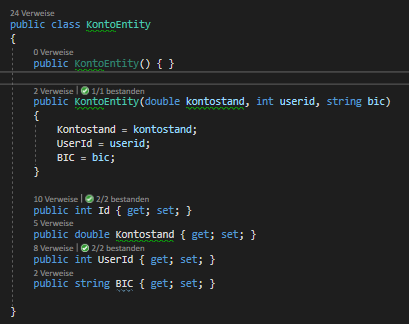
\includegraphics[width=10cm]{KontoEntity.png}}
    \caption{\label{kontoEntity} KontoEntity}
\end{figure}
\subsection{Aggregates}
Aggregate gruppieren Entities und Value Objects zu gemeinsam verwalteten Einheiten.
Aggregate helfen dabei die Komplexität der Beziehungen zwischen Objekten zu reduzieren. Die Entity im Aggregat dient als Aggregate Root Entity.
\newline Folgende Aggregate sind 
erstellt worden:
\begin{itemize}
    \item BankAggregate
    \item TransactionAggregate
\end{itemize}
Eine außenstehende Klasse muss eine Methode der Aggregate Root Entity aufrufen, sollte der innere Zustand geändert werden sollen. Dadurch wird sichergestellt, dass der Zustand immer den Domänenregeln entspricht.
\newline Das BankAggregate fasst die BankEntity und die dazugehörige Adresse zusammen. Das TransactionAggregate hält das Value Object 
für die Transaktioninfos und gibt jeder Transaktion eine Id. Hier könnte für die Transaktion noch eine TransactionEntity angelegt werden, diese würde allerdings nur die Id der Transaktion halten, weshalb sich dagegen entschieden wurde eine TransactionEntity zu erstellen. 
Weitere Informationen in der TransactionEntity zu halten macht keinen Sinn, da diese nicht änderbar sein sollen und deshalb in einem Value Object gehalten werden. Der Vollständigkeit halber sollte auch für die übrigen Entities wie UserEntity und KontoEntity ein Aggregat erstellt werden, die nur die jeweilige Entity besitzen. 
Darauf wurde jedoch verzichtet, um die Übersichtlichkeit des Projektes zu verbessern. Es kam öfters zu Verwirrungen, da bei der Benutzung des Entity Frameworks und der InMemory-Datenbank auch das Aggregat eine Id benötigt, um es zu speichern.
\newline In \ref{bankAgg} wird ein Ausschnitt aus dem BankAggregate gezeigt:
\begin{figure}[htbp]
    \centering
    \fbox{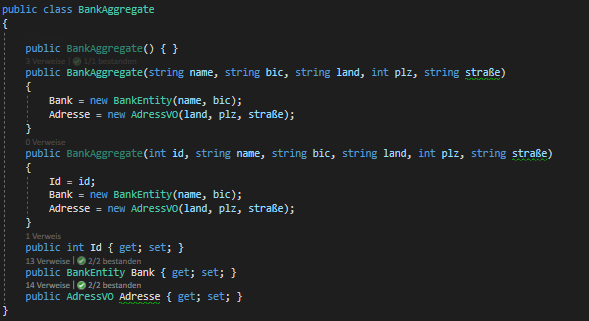
\includegraphics[width=10cm]{BankAggregate.png}}
    \caption{\label{bankAgg} BankAggregate}
\end{figure}
\subsection{Repositories}
Es wurden Repositories für User, Konto, Bank und Transaktion erstellt. Sie vermitteln zwischen der Domäne und dem Datenmodell. Innerhalb der Repositories werden Methoden zur Verfügung gestellt, 
um Aggregates aus dem Persistenzspeicher zu lesen, zu speichern oder zu löschen. Der Domain Code erhält dadurch Zugriff auf den persistenten Speicher, deren Implementierung wird der Domäne allerdings verborgen und ist somit flexibler. So wird eine Anti-Corruption-Layer zur Persistenzschicht gebildet.
Ein großer Vorteil von Repositories ist, dass zukünftig weitere Datenbanken einfach hinzugefügt oder ausgetauscht werden können, , ohne dass der Domain Code davon beeinflusst wird.
\newline Die wichtigsten Methoden eines Repository's sind diejenigen, die eine Aggregate Root Entity anhand ihrer Eigenschaften finden können. Dazu gehören beispielsweise die Funktionen eine Root Entity über ihre Id zu finden.
\newline Implementiert werden die Repositories in der Plugin-Schicht, da sie, wie bereits erwähnt, die Methoden zur Verfügung stellen um mit dem Persistenzspeicher zu arbeiten.
\newline In \ref{bankRepo} wird eines der erstellten Repositories gezeigt:
\begin{figure}[htbp]
    \centering
    \fbox{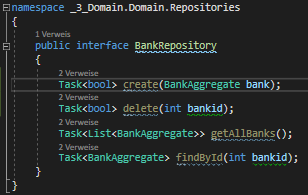
\includegraphics[width=10cm]{BankRepo.png}}
    \caption{\label{bankRepo} BankRepository}
\end{figure}
\subsection{Domain Services}
Domain Services dienen zum einen der Abbildung von komplexem Verhalten, das nicht eindeutig einer bestimmten Entity oder Value Object zugeordnet werden können und zum anderen als Definition eines \glqq Erfüllungs-Vertrages \grqq für externe Dienste, um zu verhindern, dass ein Domänenmodell nicht mit unnötiger \glqq accidental complexity \grqq belastet wird. Eine weitere wichtige Eigenschaft von Domain Services ist, dass sie selbst zustandslos sind.
\newline In diesem Projekt wurde beispielsweise ein Domain Service zur Überprüfung der Namens-, Email- und Passwortkonventionen erstellt. Dieser überprüft mit Hilfe einer Regular Expression bei Erstellung eines Benutzer, ob die übergebenen Parameter korrekt sind.
\newline In \ref{domServ} wird ein Ausschnitt des implementierten Domain Service gezeigt:
\begin{figure}[htbp]
    \centering
    \fbox{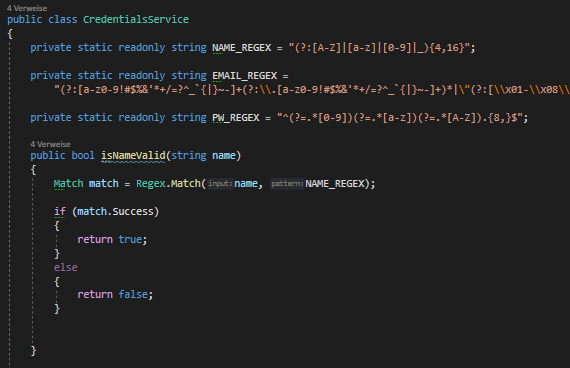
\includegraphics[width=10cm]{domServ.png}}
    \caption{\label{domServ} Ausschnitt aus CredentialsService}
\end{figure}

